\section{MCU}

The MCU is used as an I/O-processor, reading from a MicroSD card, configuring the FPGA, and feeding kernel and image data to the FPGA over an EBI bus interface. An EFM32GG is used as the MCU for the system, providing 128kB RAM, 1024kB internal flash memory and a range of modules including EBI, USART, GPIO and DMA. The board has headers connected to unused pins on the MCU, making it possible for the MCU to communicate with other devices. Figure \ref{fig:mcuOverview} shows how the components are connected.

\begin{figure}[h!]
    \includegraphics[width=\linewidth]{img/mcu_overview.png}
    \caption{Overview of the components connected to the MCU}
    \label{fig:mcuOverview}
\end{figure}

\subsection{Storage}
Due to the limited size of the MCU non-volatile memory not exceeding 1024kB, an additional larger source of data is necessary for storing files such as images and configuration files for the FPGA. A MicroSD card is used for this storage, as it gives the MCU an external storage of up to 32GB and lets the system operate independently without being connected to an external computer.

The code for interfacing the MicroSD card is based on the FAT on SD Card Application Note\cite{an0030}. The MCU communicates with the MicroSD card using SPI transfers with a USART module. FAT32 is used as a file system to make reading content from the MicroSD card more manageable, with the trade-off being increased computational overhead for the MCU. This also allows users to add and replace files without having to reprogram the MCU.

In the event of the MCU being unable to access the MicroSD card, it is possible to include kernel files and a few small images on the internal flash memory. Functionality for flashing the FPGA from the MCU will be lost because the size of the configuration files exceeds that of the internal flash memory.

The folder structure on the MicroSD card is shown in Table \ref{microsd_folder}.

\begin{table}[h!]
\centering
	\begin{tabular}{ | l | p{10cm} |}
		\hline
		Folder Name & Contents \\ \hline
		binfile & Contains binary configuration files that can be used to program the FPGA to alter its behaviour. \\ \hline
		image & Contains images that can be fed to the FPGA. Serves as a backup for the camera input. Supports 24-bit BMP files and 24-bit raw image data. \\ \hline
		kernel & Contains different kernels used for convolution. \\ \hline
	\end{tabular}
	\caption{MicroSD card folder structure}
	\label{microsd_folder}
\end{table}


\subsection{FPGA Configuration}
When the system is powered up the FPGA will not contain a configuration. To be able to use the FPGA properly, the MCU has to program it with one of the binfiles from the storage. Pins between the MCU and the FPGA are connected according to Slave Serial as described in Spartan 6 Configuration User Guide\cite{ug380} page 28. This configuration scheme relies on sending a binfile as a serial data stream using a clk pin and a single data pin. The MCU is able to reset the configuration of the FPGA at any time by setting the program pin on the FPGA low. Configuration status pins set by the FPGA informs the MCU if it is ready to be programmed, if an error occurred while programming or if the FPGA has successfully programmed.

The FPGA can also be reprogrammed later. For example when using kernels of different sizes, a configuration optimized for a specific size can be configured on the FPGA.

If the MCU is unable to read a configuration file and thus unable to flash the FPGA, it is still possible to use a JTAG header to flash manually.  

\subsection{Kernels}
Being able to change the convolution kernels while the system is running is considered an important functionality. To support this, the MCU is able to read convolution kernels from MicrodSD or the internal flash memory. 
In order to make the process of changing kernels for the system, the kernel files has a simple file structure. The kernel files consists of 8-bit values. The first byte tells the size of the kernel. For a 3x3 kernel the size will be 9. This limits us to a maximum size of 15x15 kernels. The next byte is the divisor, which is used for averaging filters. The rest of the bytes in the files are the elements of the kernel.

\clearpage % TODO: find a better way to put the wrapfigure on one page
\subsection{External Bus Interface}
%\begin{wrapfigure}[14]{r}{6cm}
%    \centering
%    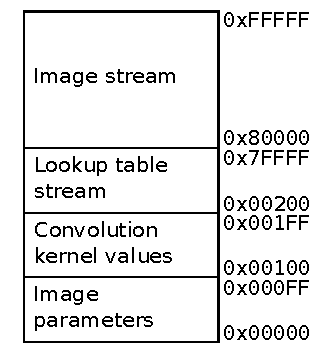
\includegraphics[]{img/EbiAddressSpace.pdf}
%    \caption{EBI Address Space}
%    \label{fig:EbiAddressSpace}
%\end{wrapfigure}
The FPGA and the MCU is connected through an EBI bus.
This interface is supported natively by the MCU and can therefore be handled by its built-in direct memory access (DMA) unit, which hopefully makes streaming video from the MCU faster, more reliable and easier to implement.

In addition to streaming video, the MCU should also control the operation of the processor.

\subsubsection{EBI Banks}
The EBI module on the MCU supports reading and writing to multiple memory banks, where each bank has its own memory space on the MCU and its own chip select signals. For the system, one bank is used access SRAM and another bank is used to communicate with the processor.

Even though the width of the EBI bus is 20-bit, only 3 addresses are used when communicating with the processor. Table \ref{ebi_processor_addresses} explains the functionality of the different adresses.

\begin{table}[h!]
\centering
	\begin{tabular}{ | l | p{10cm} |}
		\hline
		Address & Functionality \\ \hline
		0 & Data stream. Used for sending images and configuration data to the processor. \\ \hline
		1 & EBI mode override. Writing 1 to this address will give EBI access to SRAM. \\ \hline
		2 & Reset. Writing anything to this address will reset the processor. \\ \hline
		>2 & Data written to addresses larger than 2 will be ignored by the processor. \\ \hline
	\end{tabular}
	\caption{Address functionality for processor bank}
	\label{ebi_processor_addresses}
\end{table}


\subsubsection{Processor Configuration}
To configure the processor with new kernel, map and reduce values, the MCU needs to reset it. After the processor has been reset, it expects the configuration values as a data stream. The MCU then sends all of the configuration values to address 0. When the processor is fully configured, the MCU can be set to send an image stream or just wait for input.

%TODO Proper details of input stream.

\subsubsection{SRAM Access}
Instead of sending everything as a data stream to the processor, the MCU can access the image memory in SRAM. This makes it possible for the MCU to only update a part of the screen, instead of updating the whole screen every time it needs to be refreshed.

For the MCU to access SRAM it needs to enable the EBI mode override by writing 1 to address 1 on the processor bank. By doing this, the MCU will receive direct access to the SRAM through the FPGA.
The EBI bank for accessing SRAM can then be used to read and write from memory.

Writing 0 to address 1 on the processor bank will disable the EBI mode override, and resume normal operation of the processor.


\subsection{User Interface}
The system has a simple graphical user interface which is displayed on the screen. The interface has menus where it is possible to change different configuration values for the processor, such as kernels, map and reduce operators and FPGA configuration. Controlling the user interface is done with buttons, making it easier to use and removing the need for being controlled by an external computer.

The system provides four buttons for the user interface:
\begin{itemize}
	\item UP
	\item DOWN
	\item BACK
	\item OK
\end{itemize}

\subsubsection{Startup and Reset}
When the MCU is first started up or reset, it reconfigures the FPGA with a default binfile. After configuration of the FPGA, the MCU configures the processor with default values for the convolution kernel, map operation and reduce operation. The processors image input is then configured to the default input, which can be the camera input or HDMI input.

\subsubsection{Main Menu}
When pressing the BACK or the OK button, the MCU configures the processor image input to be the EBI bus and the map and reduce operations on the processor to not alter the image. An image containing the main menu of the grapical interface is then loaded from the MicroSD card and sent to the processor over the image stream. The main menu displays the following options:

\begin{itemize}
	\item Configure kernel
	\item Configure FPGA
	\item Configure map operation
	\item Configure reduce operation
	\item Select image input source
\end{itemize}

The UP and DOWN buttons are used to select an option. The OK button bring up a new menu screen listing possible options for the chosen selection. When selecting configure kernel or configure FPGA, a list of the availiable files are presented. Choosing any of the other main menu options will bring up a list of predefined choices. Selecting any of these choices will make the MCU reconfigure the processor with the new values, and go back to showing the camera image stream.


